\documentclass[prl,aps,reprint,noshowpacs,superscriptaddress,floatfix,letterpaper,longbibliography]{revtex4-2}
\usepackage{amsmath,amssymb,amsbsy,amsfonts,amsthm,bbm,bm,mathtools,mathrsfs}
\usepackage{color}
\usepackage{physics}
\usepackage{xfrac}
\usepackage[dvipsnames]{xcolor}
\definecolor{LapisLazuli}{RGB}{47, 102, 169}
\usepackage[colorlinks=true,citecolor=LapisLazuli,linkcolor=LapisLazuli,urlcolor=LapisLazuli]{hyperref}
\usepackage{empheq}
\usepackage{pgfplots}
\usepackage{stackengine}
\usepackage{relsize}
\usepackage[inline]{enumitem}
\usepackage[normalem]{ulem}
\usepackage{comment}
\usepackage{import}
\usepackage[english]{babel}
\usepackage{lipsum}  

% Macros
\newcommand{\sdc}[1]{\textcolor{blue}{[SD: #1]}}
\newcommand{\jrg}[1]{\textcolor{red}{#1}}
\newcommand{\jrgc}[1]{\textcolor{red}{[JRG: #1]}}

\begin{document}
	
	\title{Paper title here TestTestTestTestTest}  
	
	\author{Author's name}
	\author{Jason~R.~Green}
	\email[]{jason.green@umb.edu}
	\affiliation{Department of Chemistry,\
		University of Massachusetts Boston,\
		Boston, MA 02125
	}
	\affiliation{Department of Physics,\
		University of Massachusetts Boston,\
		Boston, MA 02125
	}
	\date{\today}
	
\begin{abstract}	
	Abstract goes here.
	\lipsum[1-1]
\end{abstract}

\maketitle

\section{Introduction}
Introduction here Ref~\cite{Nicholson2020}

\lipsum[2-3]

\section{Results and Discussion}
Describe your results

\begin{align}
\Delta t \bar S/n\geq k_B.
\end{align}

\lipsum[2-3]
\begin{figure}[h!]
	\centering
	\hspace*{-0.75cm}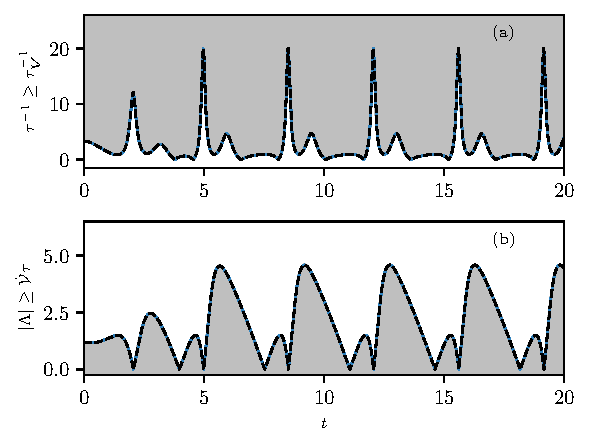
\includegraphics[width=0.45\textwidth]{sample-plot.pdf}
	\caption{Caption goes here}
	\label{fig:plot-label}
\end{figure}


\section{Conclusions}

Conclude the paper

\lipsum[2-3]

\section{Acknowledgments}
\begin{acknowledgments}
% This text is provided by the funding agency. Jason will provide.
This material is based upon work supported by the National Science Foundation under Grant No. ....

\end{acknowledgments}
\appendix

\bibliography{references}

\end{document}
